%----------------------------------------------------------------------------------------
%                   Galway-Mayo Institute of Technology (GMIT)
%                Department of Computer Science and Applied Physics
%
%                      *** Latex template for dissertations ***
%----------------------------------------------------------------------------------------

\documentclass{book}

\usepackage{wrapfig} % for wrapping images
\usepackage{graphicx} % Required for the inclusion of images
\usepackage{subcaption}
\usepackage[numbers]{natbib} % Required to change bibliography style to APA
\usepackage{amsmath} % Required for some math elements 
\usepackage{makecell}
\usepackage{eurosym}
\usepackage{tabularx}
\usepackage{pbox}
\usepackage{url}
\usepackage{hyperref}
%\usepackage[backend=biber]{biblatex}
\setlength\parindent{0pt} % Removes all indentation from paragraphs

\newcommand*{\customTitle}{\begingroup % Create the command for including the title page in thehttps://www.overleaf.com/project/5eaf58b52059020001500a63 document
\centering % Center all text
\vspace*{\baselineskip} % White space at the top of the page

\rule{\textwidth}{1.6pt}\vspace*{-\baselineskip}\vspace*{2pt} % Thick horizontal line
\rule{\textwidth}{0.4pt}\\[\baselineskip] % Thin horizontal line

%----------------------------------------------------------------------------------------
%	1) Change Dissertation Title
%----------------------------------------------------------------------------------------
{\Large BATTLE BEANS \\[2ex] 2 PLAYER CO-OP BATTLE SHOOTER FOR UNITY}\\[0.2\baselineskip] % Title
%----------------------------------------------------------------------------------------


\rule{\textwidth}{0.4pt}\vspace*{-\baselineskip}\vspace{3.2pt} % Thin horizontal line
\rule{\textwidth}{1.6pt}\\[\baselineskip] % Thick horizontal line
\scshape % Small caps \\[\baselineskip] % Tagline(s) or further description
\Large \textbf{Final Year Project}\\
\textbf{B.Sc.(Hons) in Software Development}\par % Location and year
\normalsize
\vspace*{2\baselineskip} % Whitespace between location/year and editors


%----------------------------------------------------------------------------------------
%	2) Change Student Name(s)
%----------------------------------------------------------------------------------------
{by \\ Cian Doyle \par} % Editor list
%----------------------------------------------------------------------------------------


\vspace*{2\baselineskip} % Whitespace between location/year and editors
\vfill % Whitespace between editor names and publisher logo
{\scshape \today} \\[0.3\baselineskip] % Year published
%----------------------------------------------------------------------------------------


%----------------------------------------------------------------------------------------
%	3) Change Supervisor
%----------------------------------------------------------------------------------------

{\textbf{Advised by Dr. John Healy \& Kevin O'Brien}}\par % Supervisor

{Department of Computer Science and Applied Physics Galway-Mayo Institute of Technology (GMIT)}\par % Department
%----------------------------------------------------------------------------------------


\endgroup}
\begin{document} 
\pagenumbering{gobble}
\begin{figure}
\begin{center}

\includegraphics[width=8cm,height=3.3cm,keepaspectratio]{gmit-logo} % Include the image placeholder.png
\end{center}
\end{figure}
\customTitle % This command includes the title page
\tableofcontents
\listoffigures
\pagenumbering{arabic} 



%----------------------------------------------------------------------------------------
%	4) Change Chapters
%      Write each chapter in a separate TEX file and include here
%----------------------------------------------------------------------------------------



\section*{About This Project}

\paragraph {Abstract:} Gaming today plays an expanding significant role in society. In today's society, gaming is everywhere and is hugely popular among those at a young age, those in their adulthood and even those considered to be over age pensioners are enjoying there time gaming. The reason for this is that there are a wide variety of different genres of games to suit just about any taste that a person may have. From educational purposes that can be both used in schools to teach different topics, like History and Geography to name a few, to those who are simply looking to break away from the shackles of reality by immersing themselves in another world in the shape of a video game. \par
 In recent years the rise of Indie (Independent) Developers in the video game industry has grown exponentially and shows no sign of slowing down as it is becoming easier for just about any person to create their own game with the use of the many gaming engines out there like The Unity Engine, RPG Maker Engine and Unreal Engine 4. An Indie developer is considered either a single person that works on the creation of a game or a small team of two to ten people that work on separate aspects like artwork, sounds, programming and story telling. \par
This project aims to follow the trend of Indie game developers and create something that will allow a form of escape from the stress of the real world that targets any audience, Similar to the thousands upon thousands of small fun indie games that are out there. As the author is in the is in the field of computer science that enjoyed the module of games development, this project will be completed using the knowledge gained from learning about the Unity Game Engine and will appeal to those looking to play a fun mini game that has a one versus one battle scenario. \par 
The project will be a one on one battle game with the objective to reduce the opponents life to zero or to traverse the levels to collect coins in order to gain victory.\par \bigskip

\textbf {Authors:} This project was developed as a 15 credit project by Cian Doyle, A final year student of Software Development at Galway Mayo Institute of Technology.\\

\textbf {Acknowledgements:} The author of this project would like to acknowledge and thank the project supervisors Kevin O'Brien and Dr.John Healy of Galway Mayo Institute of Technology for offering their time and advice throughout this project.
\newpage


\chapter{Introduction}
 During the first three years in GMIT (Galway Mayo Institute of Technology) we had been thought a broad range of topics from hardware to software and several different computing languages including Java, HTML, C, C\# and JavaScript to name just a few. This was done so that we the students could be ready when the time came to choose which path we would like continue in terms of a career. A part of this project is to show what has been learned through the Software development course and to put it in to practice.\par

In 2019 during the first semester of our fourth and final year, we were told that we would be doing a project that would take place over the two semesters. So in October of 2019 I began brainstorming in order to get ideas of what to do in order to start work early. Due to the fact I have always been interested in gaming and entails making your own game, I brought forward an idea to my supervisor of making a small two player versus game. With input from supervisors and from my own ideas, I was able to determine that I would use the Unity game engine to complete my project.\par
In our second semester of third year, we were given a project to do for our Mobile App Development module and this is where I first developed my interest in using the Unity game engine. I created a small endless 3D shooter game in which the player had to fight off a horde of never-ending zombies. The process of seeing my own creation become playable and fun is what really got my interest in games development and in the first semester of our final year I created a small 2D Platformer game for the Mobile Applications Development module again in which we got to experience the developer and customer side of the games development process by being given another students game idea and creating it for them using Unity. Looking at gaming and how much the gaming industry is worth, I wanted to understand it better and have a better grasp on how games are made.

\newpage


\section{Project Objectives}

As mentioned above, the main goals for this project was to gain an understanding of how games are made, the languages used to make them, the different gaming engines that are used for development and to create something light and fun to take a small getaway from the real world to have fun with friends.

This project has been divided into two parts, the research-based dissertation and the applied project. The project will be discussed in terms of the research behind it and the technologies used to build it, this being the reason that it has been split into two parts.\par
The objectives that have been set out for the dissertation are as follows: \par

\textbf {Dissertation:}

\begin{itemize}
  \item \textbf {Introducing the concept of the project:} The reader will be provided with an introduction that will describe the project and will detail its inspiration and goals.\par
  \item \textbf {Provide an understanding of Game engines:} To date, there are a vast amount of technologies available for games development, from Unity, to GameMaker and to UnrealEngine4. Exploring the different technologies I will discuss pros and cons to each and show why I felt my final decision was most suitable for my final project. \par
  \item \textbf {Describe the development of the applied project:} This dissertation aims to give you, the reader, a comprehensive guide into the process of development from the first steps of the initial researching through to the finalized end product. I will describe the approach taken to the applied project, which will include methodologies and technologies used with the design of the games design. For the conclusion I will be discussing any issues that occurred during development, how I went about solving them and what would i have done differently or what I would have liked to of added in future development.\par
\end{itemize}


\textbf {Applied Project:}

\begin{itemize}
  \item \textbf {Make a simple, yet fun to play game:} The project will be able to provide the user with a relatively fun and slightly competitive experience to play with friends or family that can be ran on any computer using Windows. \par
  \item \textbf {Dive into deeper learning into using game engines:} For the purpose of expanding my knowledge and skill-set, the development will be conducted using technologies that have been previously used in the Software Development course. This will further expand on what I have been thought, further progressing the learning outcomes of the modules.\par
  \item \textbf {Complete the project using an efficient and effective approach:} The project will be developed using appropriate tools and methodologies. With the intention of maximising efficiency and effectiveness, a record will be kept of all issues that arose and how they were fixed or why the issues were taken out of the final build.\par
\end{itemize}



\section{Metrics For Success And Failure}

In order for the development of the game to be in a controlled manner along with being able to manage progress in early development, it was vital that metrics were outlined for success or failure. Doing this enabled to keep track of what I wanted to achieve. The simplified list of metrics for the success of the project are as followed:

\begin{itemize}
  \item \textbf {Make a simple, yet fun to play game:} To measure this through different stages of development, I gave my friends outside of the computer science course and fellow students in my year playable versions of levels that I had made in order to gain feedback from different perspectives. \par
  \item \textbf {Make continuous builds to test as the project develops:} Continuously looking for bugs and errors through making build versions of the game to test what, if anything, comes up as an error.
\end{itemize}


\section{An Outline of each chapter}

\paragraph{} This paper has been organised into different chapters with each chapter containing different details in regards to the various aspects of the project. Each of these chapters will be briefly outlined in the following sub-sections.

\subsection{Methodology}
In chapter 2 I will explore what approaches I followed to plan, organize, manage and develop the project. This is where I will discuss the methodologies that were used in order to complete the development of the project along with the research as well as to why they were implemented. The methodology section will provide the reader with an insight as to how the project went from the research to the final product.

\subsection{Technology Review}
In chapter 3 I will cover the technical side of the project which will consist of looking back on the technologies that made up the final version of the project. I will go on to explain explain the different types of technologies that were added and how they were implemented through the project. I will also be explaining why I used the technologies that I included as well as why I decided against using certain technologies as well as the benefits to using one over the other.

\subsection{System Design}
In this chapter I will discuss the architecture and design of the Battle Beans game. This will consist of code snippets and diagrams to help show a basic understanding of the games design. The chapter will begin with a brief overview of the flow the design followed by an in-depth view of what went into making the game and how each feature functions

\subsection{System Evaluation}
This chapter will evaluate the software developed in the project. It will be evaluated in the areas of robustness, testing and scalability as well as a measurement of the results of the final build versus the objectives set out in the beginning. I will also discuss ways i could of improved what was used.

\subsection{Conclusion}
To conclude, a brief review of the overall final project and goals of the project will be outlined. Also to be included is what I would add in further future developments, a final analysis, as well as a review of the discoveries made while researching and the skills learned in the process. For a finish I will leave a brief discussion of my experience working on the project.\cite{}

\section{Requirement Specification}

Below is a list of requirements I made for the project: \par \bigskip
\textbf {Requirements:}

\begin{itemize}
  \item  Be able to load different levels \par
  \item  Be able to determine a winner through score \par
  \item  Allow player to shoot. \par
  \item  Allow Game to end when timer reaches zero \par
  \item  Be able to end game as a draw if scores are equal after the timer reaches zero \par
  \item  Be able to jump through the bottom of a platform \par
  \item  Players can pick up coins to add to score \par
  \item  Players can pick up health drops only if they have lost health \par
  \item  Health items spawn in intervals of 15 seconds  \par
  \item  Coins spawn in intervals of 5 seconds \par
\end{itemize}






\chapter{Methodologies}
 In this chapter, I will be discussing the methodologies used in the project. Throughout the four years in GMIT, we were always told through several modules that software development methodologies and the choosing of the most suitable methodology for a given project were of extreme importance in any company that one would work in. Due to this, I researched different methodologies which I could use for my project, seeing the positives and negatives of each one. After researching each one I decided to go with using Agile as my main methodology. I felt this would be the best method to suit the development and it is also a widely used methodology in organizations around the world.

\section{Agile Development}
\begin{wrapfigure}{r}{0.25\textwidth} %this figure will be at the right
    \centering
    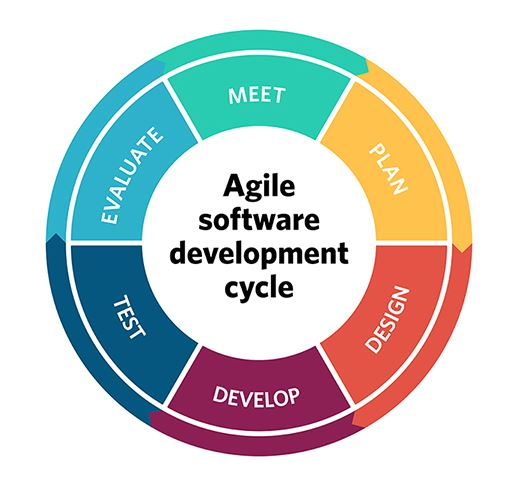
\includegraphics[width=0.3\textwidth]{Images/agile-software-development.jpg}
    \caption{Agile Cycle.}
  \label{fig:Agile Cycle}
\end{wrapfigure}
 Agile Development is a concept that allows that allows the product to be delivered to the customer in incremental releases as well as also being extremely flexible, which allows change to the requirements and allows the scope of the project to be increased without inflicting consequences on the design.

 The project contained Three main stages, research, design and implementation. For each stage I applied an agile like approach in order to complete them. I felt agile was best suited for the project as it allows for plenty of flexibility and allows the software to be delivered incrementally. I used a scrum like approach for each of the research, design and development processes. Scrum is an agile framework where members break their work into actions that are able to be completed within sprints, which are timed iterations, which usually last two weeks but can last up to a month long. Progress is then tracked and re-planned in meetings. \cite{AboutAgile}

\newpage

\subsection{Sprints}

A Sprint is a timed iteration of the continuous development cycle with a scrum being a discussion in the style of a meeting used to gain feedback. During the development of the project, my default sprint was a two week cycle after each meeting with my supervisor where I would plan what I would like to get done in the two week window. \cite{Sprints}

\begin{figure}[h]
  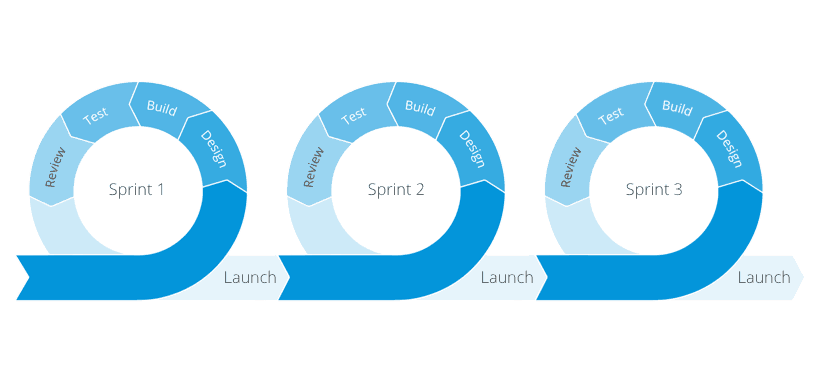
\includegraphics[width=\linewidth]{Images/AgileSprint.png}
  \caption{Sprint Cycle.}
  \label{fig:Sprint Cycle}
\end{figure}


\subsection{Meetings}

During the course of the college year, weekly meetings were held with a project supervisor to see how we were getting on with the project with initial meetings being used to brainstorm our ideas and get feedback on them. The meetings consisted of updates of our progress along with feedback on that progress, any advice or help was given to us if needed, and plans were put into place of what we would have done for the following meeting. If however a meeting could not be made, a simple email outlining what had been done and what was to be done next was sent to the supervisor to which they would promptly reply to giving their best advice and feedback.
\newpage

\section{Version Control}
\begin{figure}[h]
  
\includegraphics[width=\linewidth]{Images/GitHub.png}
  \caption{GitHub.}
  \label{fig:GitHub}
\end{figure}
For this project, I decided on using the online web-based GitHub Source Control Software. GitHub is a development platform which allows its users to use several collaboration features such as bug tracking in its issues section, task management, and a wiki for every project. These items were very useful when it came to the development of the project. GitHub is considered one of the most popular version control management services in the world and one we have used in the Software Development for the duration of the course for our project submissions. 
GitHub enabled me to be able to store both my dissertation and my project's repository. The main function allowed me to commit the work to repositories, allowing me to be able to get a previous  working version of the project. This was especially handy in case something happened where the project was broken and I couldn't fix it. This would allow me to clone the previously known working project and work again from that version. \cite{AboutGitHub}

\section{Technology Choice}
After researching Games development and what type of game I would be designing, I came to a conclusion as to what language I would be using and which game development software I would be using for the completion of my project. I decided on using the Unity game engine to develop my game and to use the C\# language to program the game. These choices were based on my previous experience in using both during the course of my 4 years in the Software Development course. Along with these I used Visual Studio Code and the image editor GIMP. Each of these technologies will be explained further in the Technology Review chapter.
\chapter{Technology Review}
In this chapter, I will be taking a look at all the technologies used to make up the final version of the project. I will be discussing what each of the technologies used for images, coding and games development are and what each of their purpose is in the project. For this, I will be going over why I used each of the technologies along with discussing the similar versions of them and why I chose not to use these other versions.

\section{Game Engines}
In this section I will be discussing each of the game engines I at before I decided on which one I was going to use. These include the Unity Game engine and the Unreal Engine 4. I will be discussing their features as well as why I thought they would be a good or bad engine to use for the project in terms of did they have the features that I required to meet my objectives and how user friendly they were to those ranging from beginners to those who are experts in the field of games development.\cite{GameEngines}
\newpage
\subsection{Unity Engine}
\begin{figure}[h]
  
\includegraphics[width=\linewidth]{Images/UnityLogo.png}
  \caption{Unity.}
  \label{fig:Unity}
\end{figure}
\bigskip


Unity is a cross-platform game engine which was first announced and released for free in June of 2005 at Apple Inc.'s Worldwide Developers Conference as a Mac-OS X exclusive game engine, which later became available for other systems like windows. As it is cross-platform, this means that any game you make in it can be played on any console or computer such as the Xbox One, PlayStation 4, Windows OS, Linux OS and Android. The engine can produce 3-Dimensional as well as 2-Dimensional games, Virtual Reality Games and Augmented Reality Games and mainly uses the C\# scripting language. During the last 2 years of the Software Development course, this engine was used to teach us Mobile App Development where we developed games on it. I have used this engine to create 3D and 2D games from both what I have been thought in class as well as using Unity's own online lessons which release on the regular when ever a new version of the software comes out. However, even if what you want to learn how to do is not available on the lessons section on their website yet, there are hundreds of YouTube tutorials out there from the massive community of people who use this engine. 
Unity also comes with its own asset store which people can put up on the asset store for free or for a small or large fee. The assets can be anything form 3D or 2D character or level designs, level and game music and also packages like Text Mesh Pro which makes a more crisp looking text than the one that Unity has as a default, which I will touch on more later on.
Unity also has an impressive library of games made using their engine such as the multi-award winning title "Ori and The Blind Forest" which is a 3D sidescroller adventure game and which has since produced a sequel titled "Ori and the Will of the Wisps" in which it has done equally as well as its predecessor.\cite{Unity}
\newpage

\subsection{Unreal Engine(UE4)}
\begin{figure}[h]
  
\includegraphics[width=\linewidth]{Images/Unreal-Engine-Logo.png}
  \caption{Unreal.}
  \label{fig:Unreal}
\end{figure}
\bigskip

Unreal Engine is a game engine developed by Epic Games, who in recent times has become well known due to their release of the popular battle royal title "Fortnite". It was first showcased in 1998 to be used in development for FPS(First-Person Shooter) games, but has since been used successfully in genres like platformers, fighting games and other RPGS(Role-Playing games). The current version, Unreal Engine 4, was originally released in 2014 as a subscriptions service with the first game released being a 3D Horror game Called "Daylight" but later became free to download the following year with its source code being available on GitHub. Unreal Engine uses the C++ language to develop its games. Similar to the Unity engine Unreal offers its own asset store, the Unreal Engine Marketplace, where users can buy art, character models, sounds and environments to name a few, along with tutorials and other guides on how to make your desired game.
Although it is possible to make 2D games on the Unreal Engine 4 with the project set up for 2D side-scroller now available, it was originally designed for it's main clear focus  on that of 3D graphics and shaders. To take "Bloodstained: Ritual of the Night" as an example of the capabilities of Unreal Engine 4s 2D development as you can see from figure \ref{fig:Bloodstained} that it has 3D models working on a 2D landscape.\cite{UnrealEngine4}

\begin{figure}[h]
  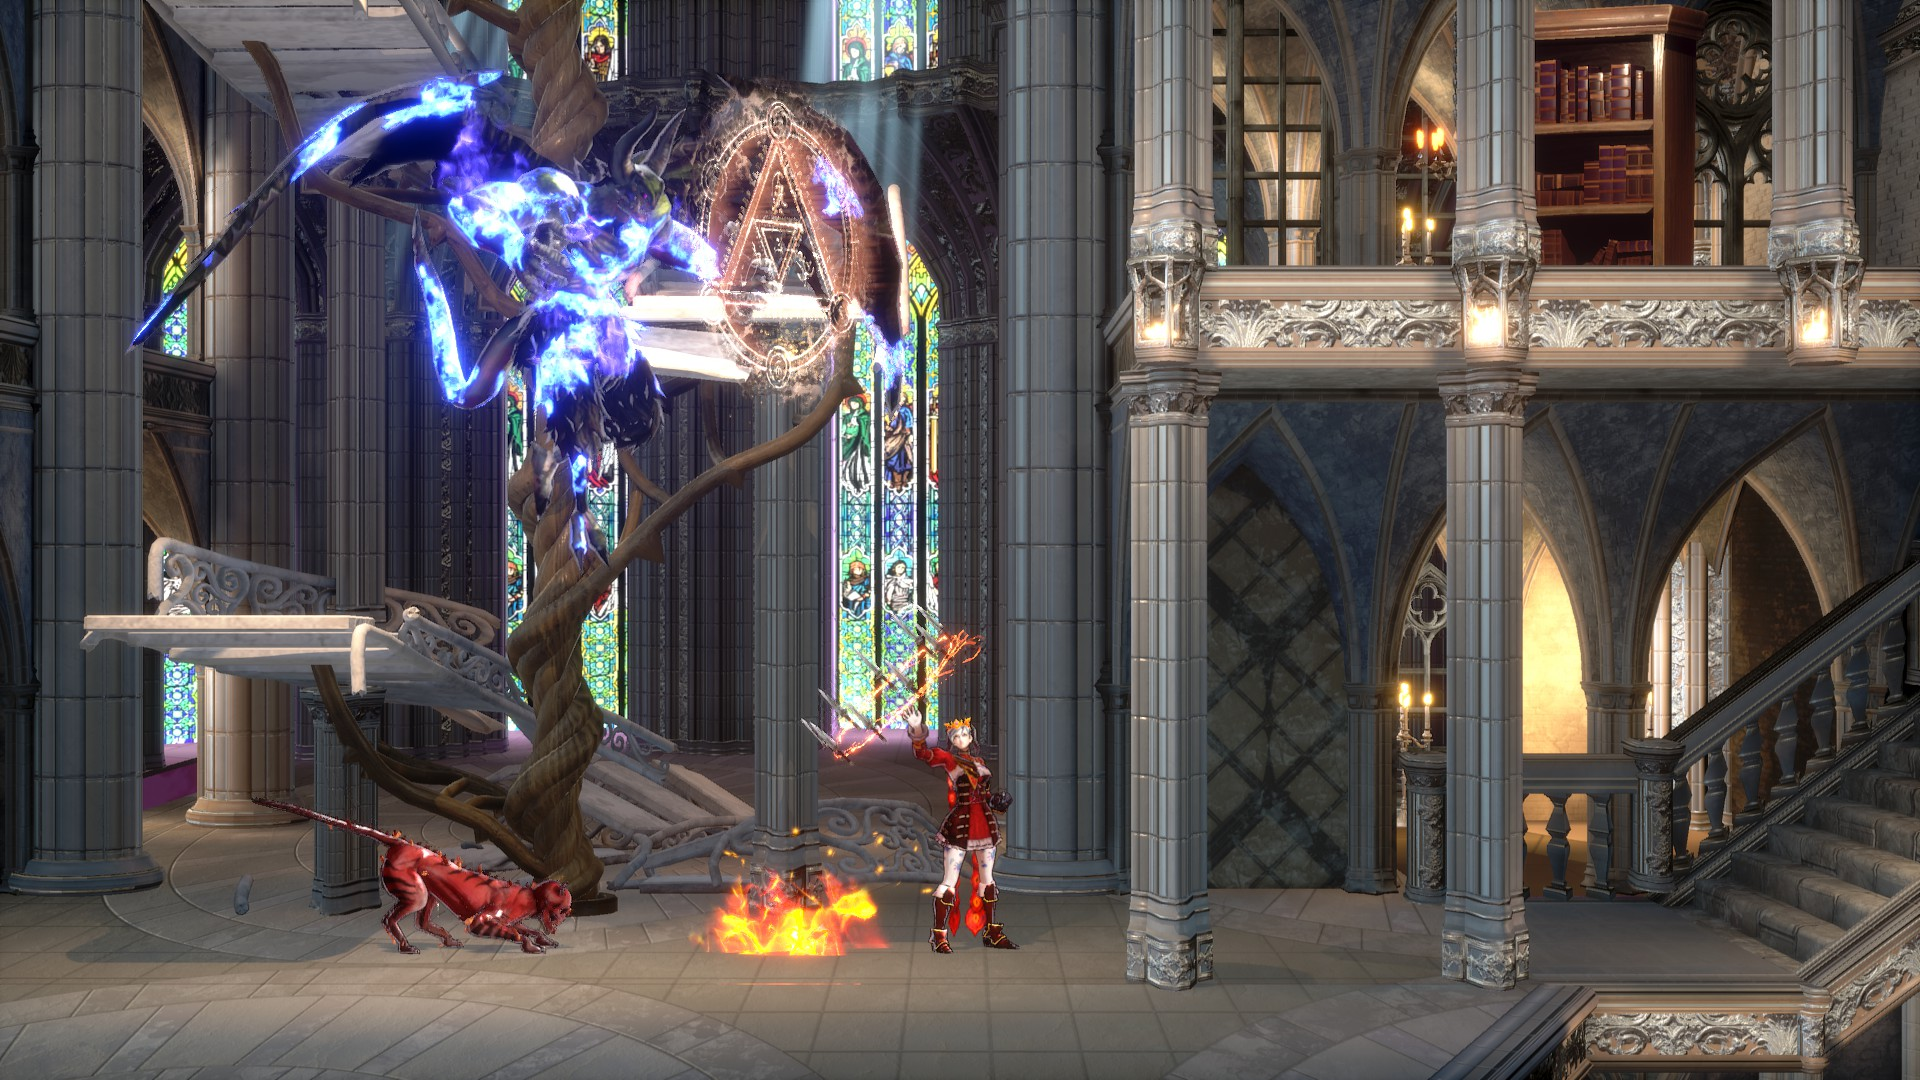
\includegraphics[width=\linewidth]{Images/Bloodstained-1080.jpg}
  \caption{Bloodstained.}
  \label{fig:Bloodstained}
\end{figure}

\newpage
\subsection{Unity Engine or Unreal Engine 4?}
\begin{figure}[h]
  
\includegraphics[width=\linewidth]{Images/UnrealVSUnity.jpg}
  \caption{Unreal vs Unity.}
  \label{fig:Unreal vs Unity}
\end{figure}
\bigskip

For this project, I had an early mindset that I wanted to create a 2-Dimensional game as I find it is a lot easier for people, myself included, that are not exactly the best artists or designers to create something that looks visually decent compared to having to learn how to use 3d modeling software's like Blender, which is used for creating 3d models, in order to create the level design and the character design. In order for me to use the Unreal Engine, I felt that after researching on it I came to the conclusion that it would not meet my requirements in order to create a 2D game as although it is possible to make a 2D game, it is mainly used for the creation of 3D games. Unreal Engine is also an engine that offers very high visuals, which means that it is much more suited to make a high end games more suited to big games development companies over a single person making a game.
Unity is more widely used for small teams or a single person making a small to medium scale games, although it is possible to make a high end large scale game, it is more suited to the small teams or singular developers. As well as this, Unity for me seemed much more user friendly as when you click to start a new project, it will give you an option to start a new 2D project and will take it as you are using 2D features for the build. I felt as though it was easier to find exactly what I was looking for when I searched online or on YouTube for ways to do certain things related to 2D development than searching for how to do it on the Unreal Engine as there was a lot of examples out there and even Unity's forum was full of guides and lessons on how to add features such as 2D level designing, background layer designs and enemy AI tracking to name a few.
To conclude, Unity was the game engine I went for, not only because I felt it met my requirements for making a 2D game, but because of the fact Unity mainly uses C\# as its main language over Unreal 4's C++ language. This is not to say that the C\# is better than the C++ language, but I felt that as I have gained experience in using the C\# language through modules in the Software development course that it would be better for me to expand on what I already knew and what I found that I have an interest in. I also chose Unity because since I first used it back in my second year for a project where I made a short shooter game, I found it very user friendly and relatively easy to learn all of its features through its online learning course and found the C\# language easier and more interesting to learn for me compared to other languages like Java, C++, HTML, etc.\cite{UnityVUnreal}

\newpage

\section{Packages}
The following section will discuss the packages used in unity for the development of the game. Packages are collections of files and data from Unity projects, or elements of projects, which are compressed and stored in one file, similar to Zip files. Like Zip files, a package maintains its original directory structure when it is unpacked, as well as meta-data about assets (such as import settings and links to other assets). For my project I used the packages TextMesh Pro for the use of text in my UI.\cite{UnityPackages}

\subsection{TextMeshPro}
The TextMesh Pro package in Unity is used as a replacement for Unity's standard UI Text and Text Mesh. It uses advanced Text Rendering and custom text shaders which allows for visual quality improvements in the text while also allowing users to put there own style of text styling and texturing. It can also enable users more control over text formatting and layout features such as word, line and paragraph spacing.\cite{TMPRO}

\begin{figure}[h]
  
\includegraphics[width=\linewidth]{Images/TMProTopvStandardBottom.PNG}
  \caption{TMP Pro(Top) vs Standard Text(Bottom).}
  \label{fig:TMP V Text}
\end{figure}




\section{Sprite Editors/Creators}

In this section I will be going through which image creation software I used in order to create the sprites that I needed for my character designs, level design and other general things like health items or collectables. For this, I looked into different Image editors like Inkscape, Krita, Adobe Photoshop and Gimp and decided to narrow it down to Gimp and Photoshop as I have had past experience in both of them. I will discuss both in terms of how user friendly they are and did they meet the requirements that I needed in order to create the art sprites for my game also taking into to consideration that drawing would not be my strong point.
\newpage

\subsection{Gimp}
\begin{figure}[h]
  
\includegraphics[width=\linewidth]{Images/gimp-logo.png}
  \caption{Gimp.}
  \label{fig:Gimp}
\end{figure}
Gimp(GNU Image Manipulation Program) is a open-source raster graphics editor that can be downloaded for free online. It is has many capabilities such as a photo retouching program, a online batch processing system, a image format converter and it can be used as a simple paint program to name just a few of its features. It's first version was released in back in 1996 being ported to windows operating system in 1997. GIMP is considered a good alternative to Adobe Photoshop as it is a free to use software with no subscription fee. In terms of video game development, GIMP is plenty powerful enough to support art for games as it was used to create nearly all the artwork for "Lucas the Game" which was made back in 2014 with the developer Timothy Courtney stating, "GIMP is a powerful tool, fully capable of large professional projects, such as video games."
GIMP is also capable of producing animations by using it's GIMP Animation Package(GAP) which is a plug-in for creating animations on the software. It can save and export animations in several formats including the most popular and widely used GIF and AVI formats. The GIMP website also offers plenty of tutorials available through its website where it teaches beginners how to start using the software, how to edit photo's such as converting to black and white, tone mapping with colours and exposure, painting tutorials and programming tutorials to name a few. It also has a long list of video tutorials available on YouTube ranging from beginners to experts.
Overall GIMP is a very user friendly image editing software that is only made better by the fact that it is free to use.\cite{GIMP},\cite{GIMPTutorial}
\newpage

\subsection{Adobe Photoshop}
\begin{figure}[h]
  
\includegraphics[width=\linewidth]{Images/adobe-photoshop.jpg}
  \caption{Adobe Photoshop.}
  \label{fig:Photoshop}
\end{figure}
Adobe Photoshop is a raster graphics editor developed and published by Adobe Inc. that was released in April of 1990. The software has become an industry standard for raster graphics editing and digital art. It is widely used by those in games development to produce the art for the games. Photoshop can compose and edit photos using multiple layers and several colour models such as RGB and duotone. Photoshop also boasts its own file formats, PSD and PSB, to support those features. A PSD(Photoshop Document) file contains a maximum of thirty thousand pixels for width and height while also allowing for a file length limit of 2 gigabytes, which is plenty big for just about any project. The other file format, PSB(Photoshop Big), is a larger version of the PSD format as it extends the pixels allowed to 300,000 pixels and extends the file limit to 4 exabytes, which totals to a massive 4000 gigabytes. Photoshop offers plenty in terms of video editing using video file formats such as MOV and MPEG-4 as well as capabilities to transform 2D elements of artwork to easily become 3D with a click of a button. Photoshop has reached such a height of popularity that it has even become a verb, as most people who see an image that has clearly been edited would state "That image has been Photoshopped" instead of simply saying it's been edited.
The Adobe website offers plenty of tutorials to both beginners and those who are experienced by being able to separate into beginner lessons, where you learn the basics like getting to now Photoshop, and experienced lessons like how to work on Photoshop using a tablet such as an iPad. Even if there is something that cant be found through their website, there are hundreds of tutorials available online and through YouTube.
Photoshop is not free however, as it charges a monthly subscription in order to use its services ranging from  \EUR{12.29} per month to  \EUR{24.59} per month. There is currently a cheaper price available to students and teachers of \EUR{19.99} per month.\cite{AdobePhotoshop}\cite{AboutAdobePhotoshop}

\subsection{Gimp or Adobe Photoshop?}


As I have stated previously, I wanted to create a simple 2D design type of game which would not require a lot of skill in terms of art and I took this into account while researching which image editor software to use. Early on I ruled out using Inkscape and Krita as even though they seemed like good tools, I had previous experience in both GIMP and Adobe Photoshop so I decided to stick to what I knew and work on further expanding my knowledge of what was familiar. Both Gimp and Photoshop are fantastic Image editor software's but the ultimate turning point on choosing one over the other came down to the price and my prior knowledge.
Due to this I decided to go with the free software GIMP over the subscription service of Photoshop. Although Photoshop is the more widely known software, the subscription fee turned me away from it as GIMP, being free, has more than enough tools in it for what I needed to make the artwork for my game. Along with this reasoning was the fact that I have used GIMP far more than I have used Photoshop so i wanted to stick to what I was more familiar with and further expand my knowledge on it for any future projects I intend to create in the future. For two of my previous projects in the software development course where developed a game, I used the GIMP software in order to create the artwork, this being another reason I was being pulled toward using GIMP. This is no in way saying that GIMP is a better software over Photoshop, as personally I think that Photoshop does seem to be the better software after researching and using both it and GIMP. However, for the purpose of making this game, I felt that GIMP was capable of providing me with exactly what I needed for the games artwork, without having to go paying for a subscription fee like Photoshop.\cite{AdobePhotoshopVGIMP},\cite{GIMP},\cite{AdobePhotoshop}
\begin{figure}[h]
  
\includegraphics[width=\linewidth]{Images/GimpVphotoshop.jpg}
  \caption{Gimp vs Photoshop.}
  \label{fig:GimpVPhoto}
\end{figure}


\section{Languages}

\subsection{C Sharp (C\#)}

\begin{figure}[h]
  
\includegraphics[scale=.5]{Images/C-sharp-logo.jpg}
  \caption{C\#.}
  \label{fig:C-Sharp}
\end{figure}

C\# is a general purpose, multi-paradigm programming language that has strong typing, functional, generic, object-oriented class based and component-oriented programming disciplines. Developed in 2000 by Microsoft, it is a programming language designed for the Common Language Infrastructure(CLI), which is an open specification developed by Microsoft. The C\# language is one of the main programming languages that is used in the development of a Unity project. Below is an example of a C\# script made for Unity.\cite{CSharp}
\begin{figure}[h]
  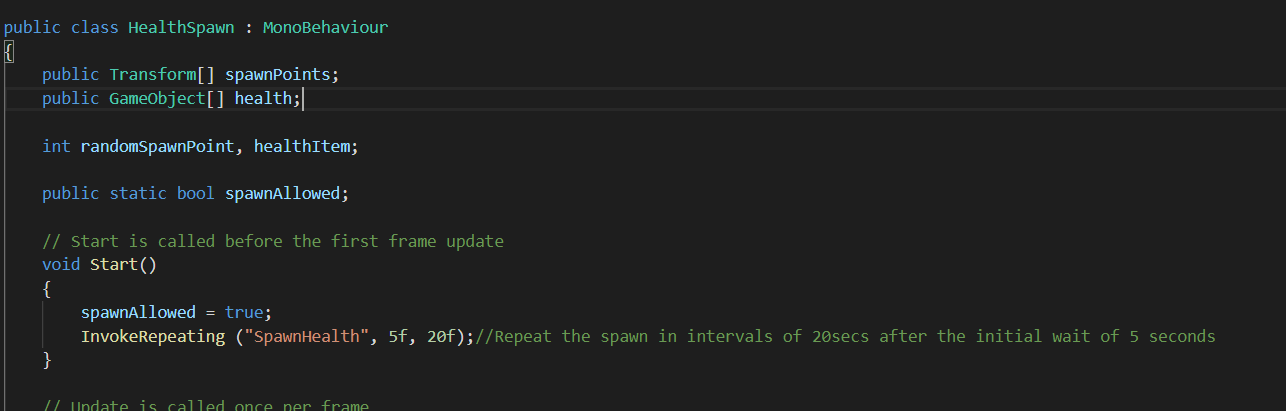
\includegraphics[width=\linewidth]{Images/C-Sharp-Example.PNG}
\newpage
  \label{fig:C-Sharp Example}
\end{figure}

\newpage
\subsection{\LaTeX}
\LaTeX \space is a text processor that is built around a markup language, which is similar to HTML.
Like HTML, \LaTeX \space uses tags to define a command or an action to display the text in a certain way. Tags are only seen in the source of the document will be hidden when the document gets compiled into the format of a PDF, see figure \ref{fig:LaTeXExample}
\begin{figure}[h]
  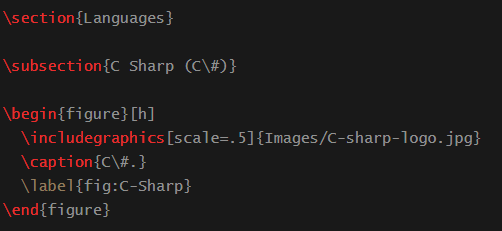
\includegraphics[width=\linewidth]{Images/Latex-example.PNG}
  \caption{LaTeX Example.}
  \label{fig:LaTeXExample}
\end{figure}
\bigskip
\newline
\LaTeX \space then compiles the text into a document like the PDF you are reading right now. It then renders the chapter, the section, the sub section and compiles it into the table of contents.\cite{LaTeX}

\newpage

\section{Other Software Used}
\subsection{Visual Studio Code}
Visual Studio Code is a source-code editor developed by Microsoft for Windows, Linux and MacOS. It comes with support for debugging, embedded Git control, syntax highlighting, intelligent code completion and code refactoring included. It has customizable features such as the editor's theme, preferences and keyboard shortcuts. The reason I used this was because it was exactly what I needed as Visual Studio Code offers specialized extensions that make developing with the C\# language much better.\cite{VSCode}, 
\begin{figure}[h]
  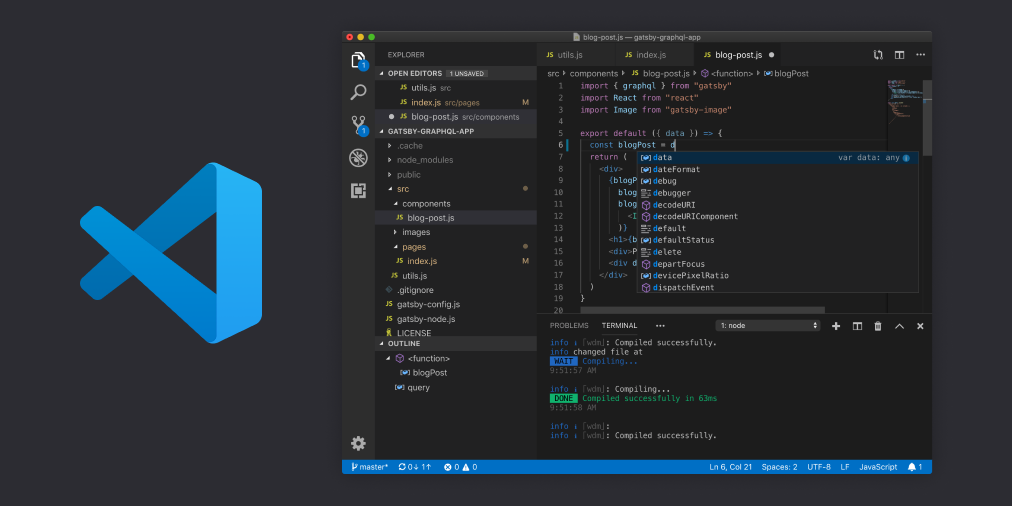
\includegraphics[width=\linewidth]{Images/VSCode.png}
  \caption{Visual Studio Code View.}
  \label{fig:VSCode}
\end{figure}
\chapter{System Design}
In this chapter, I will be discussing the overall design of the levels and UI elements in the game along with going through all the C\# scripts that I used in the game.I will show code snippets and game screenshots to explain the design of the project and how everything works. I will be breaking this chapter into three parts, Level design, coding and the final build, Firstly for the level design, I will be showing screenshots of early design ideas and why i chose not to include some of the early ideas. I will then look at the  c\# scripts used to make the game function and how Unity uses the scripts. Lastly i will be showing screenshots and giving descriptions of each on what the final build looks like. The final build will be what the users will be interacting with in order to play the game.

\section{Game Design}
In this section I will be discussing the early stage development designs for the levels and the final level designs used. Also included is the characters and scenes that never made it into the final builds as well as reasons for not including them, along with the final character designs.

\subsection{Early Designs}
During the early stages of development, I had several ideas for the game which in the end never made it into final production. These included level designs, character designs, character selection screens and different menu layouts. The reason for these not making the final product was due to either me coming up with a better idea than them or feeling that I did not want to include them in the final build. Below are all shots of the sketches of early level designs, character designs as well as a concept for a character selection screen.

\begin{figure}
\centering
\begin{subfigure}{.5\textwidth}
\centering
  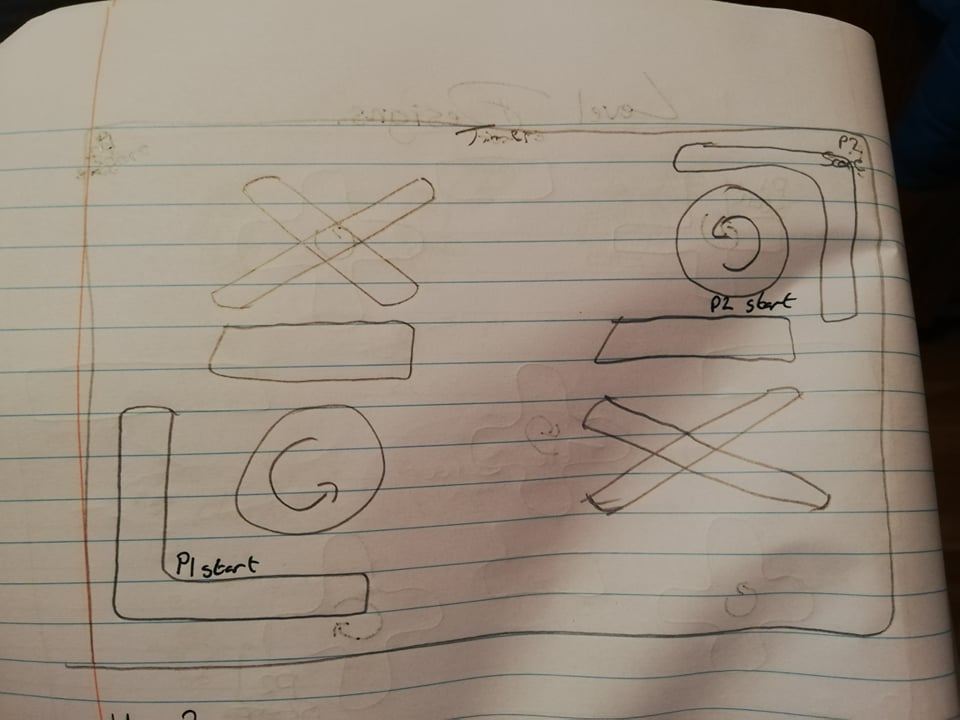
\includegraphics[width= 1\linewidth]{Images/Leveldesign1.jpg}
  \caption{Level Concept 1.}
  \label{fig:Level1 Concept}
\end{subfigure}%
\begin{subfigure}{.5\textwidth}
\centering
  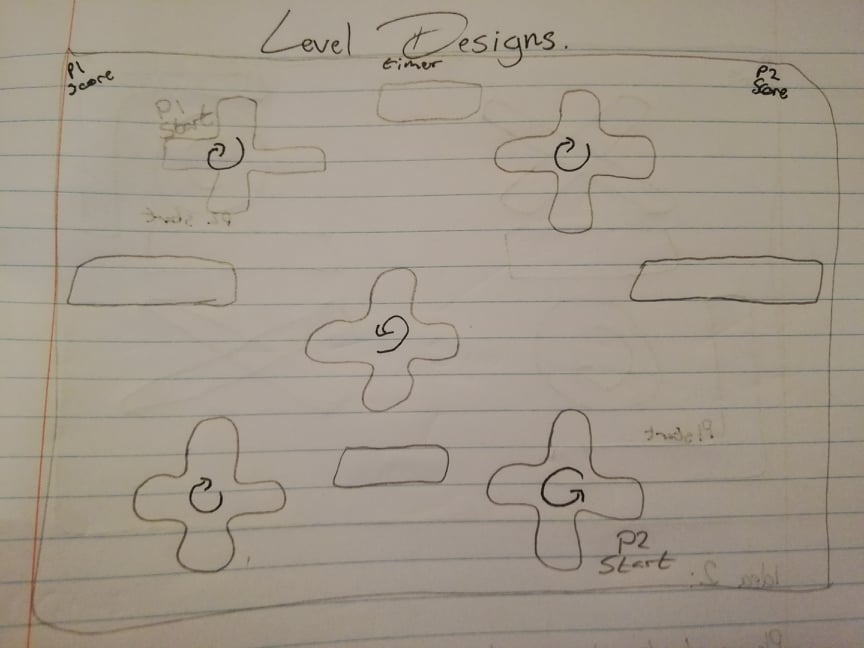
\includegraphics[width= 1\linewidth]{Images/Leveldesign2.jpg}
  \caption{Level Concept 2.}
  \label{fig:Level2 Concept}
  \end{subfigure}%
  \newline
\begin{subfigure}{.5\textwidth}
\centering
  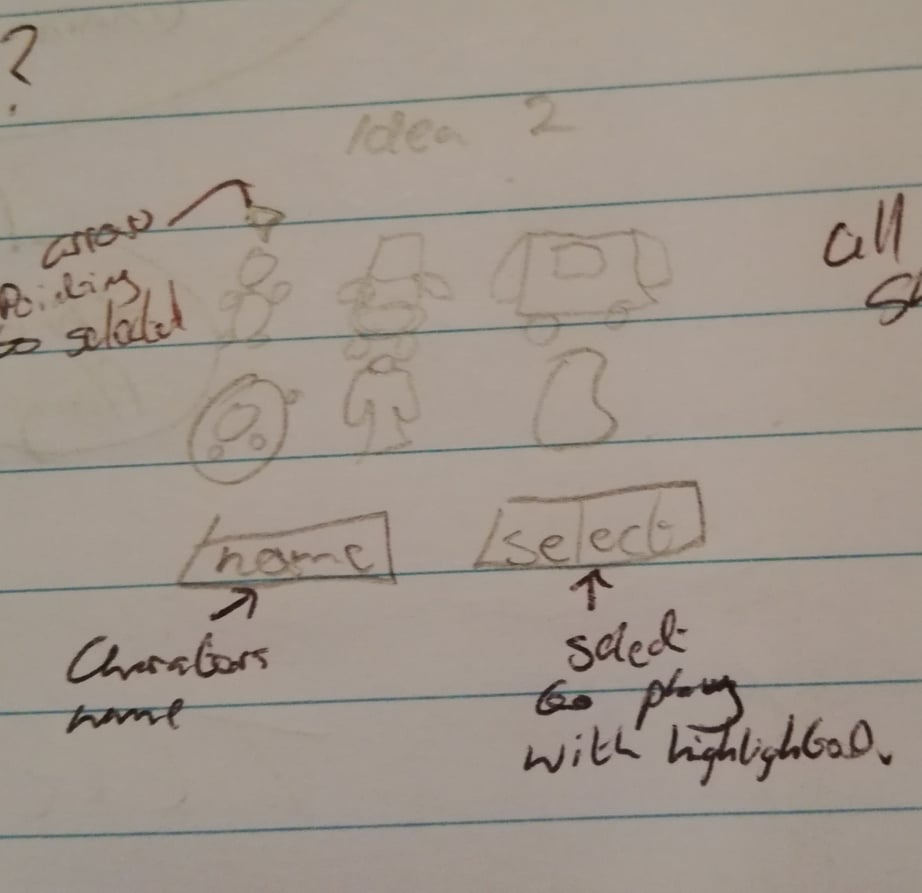
\includegraphics[width= 1\linewidth]{Images/CharacterSelectionIdea.jpg}
  \caption{Character Selection Idea 1.}
  \label{fig:CharacterSelectionIdea}
  \end{subfigure}%
\begin{subfigure}{.5\textwidth}
\centering
  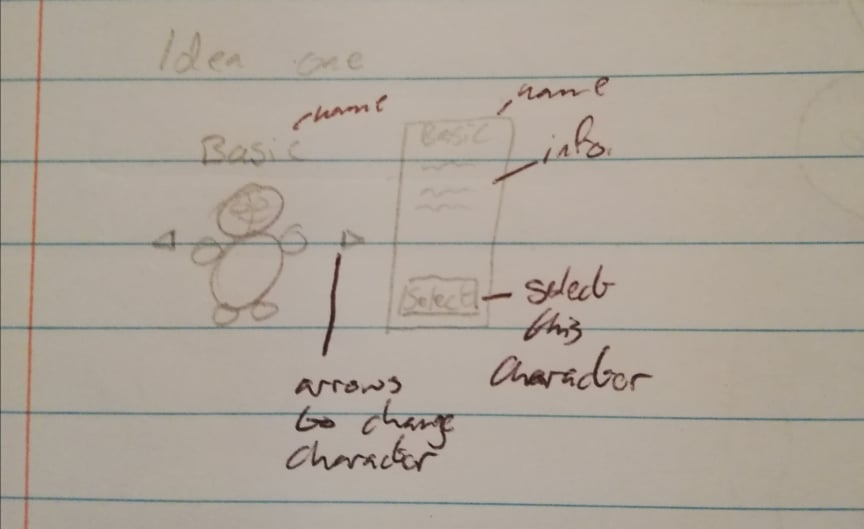
\includegraphics[width= 1\linewidth]{Images/CharacterSelectionIdea2.jpg}
  \caption{Character Selection Idea 2.}
  \label{fig:CharacterSelectionIdea2}
  \end{subfigure}%
  \newline
\begin{subfigure}{.5\textwidth}
\centering
  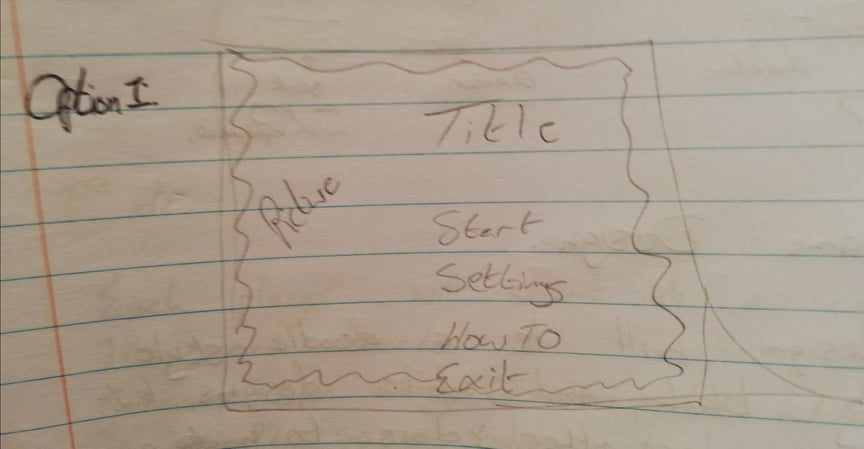
\includegraphics[width= 1\linewidth]{Images/MenuIdea.jpg}
  \caption{Menu Idea 1.}
  \label{fig:MenuIdea1}
  \end{subfigure}%
\begin{subfigure}{.5\textwidth}
\centering
  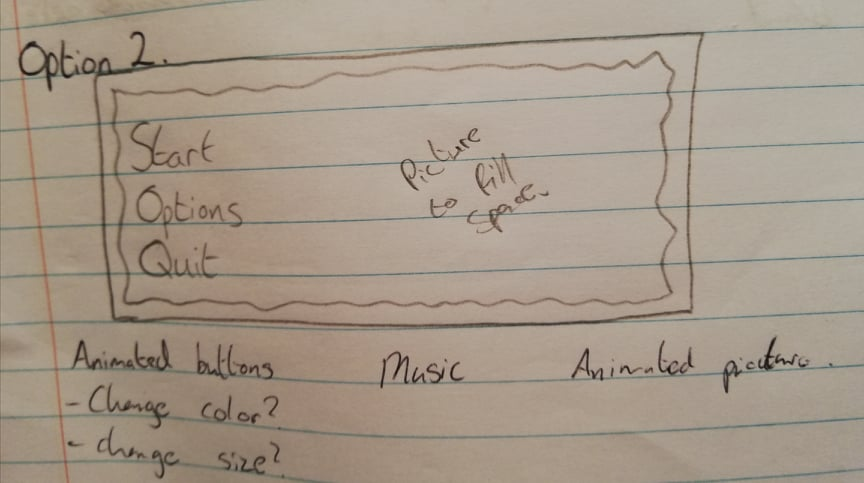
\includegraphics[width= 1\linewidth]{Images/MenuIdea2.jpg}
  \caption{Menu Idea 2.}
  \label{fig:MenuIdea2}
  \end{subfigure}%
\end{figure}

\newpage
Originally I had planned on doing a character selection screen for my game, see figure \ref{fig:CharacterSelectionIdea} and figure \ref{fig:CharacterSelectionIdea2} where you could choose to use different types of characters that would have variant types of boosts like better speed, stronger hits and higher jumps but after researching on it I came to the conclusion that because of the level designs it would run the risk of having overpowered characters like the higher jump character being able to escape the other character too quickly making it very difficult for the other player to shoot him. In the end I decided to take this idea out of the game altogether to allow for an even playing field of just two characters that boast the same stats in terms of speed, jumping and shot power.

\section{Menu Designs}
\begin{figure}[h]
\centering
  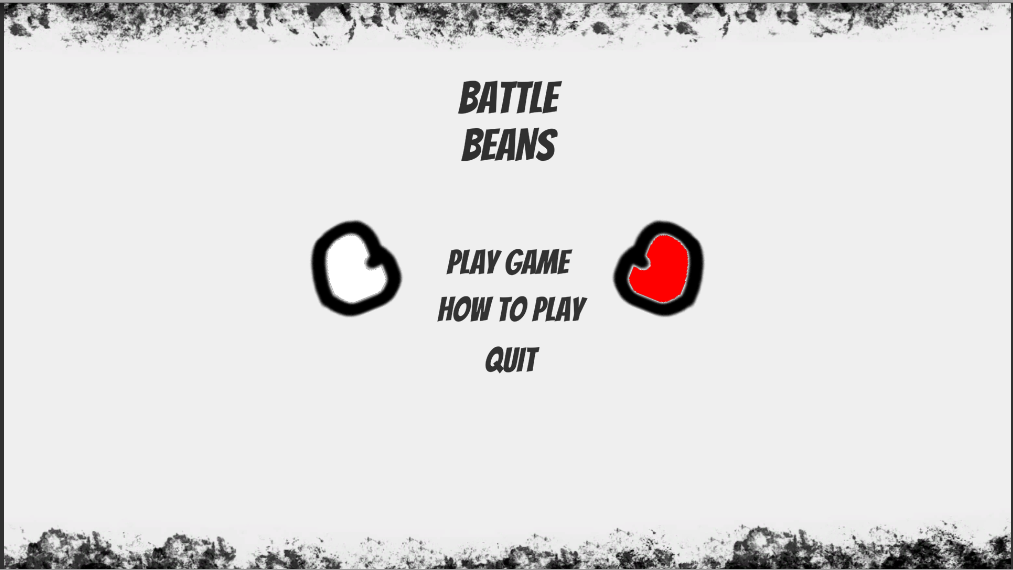
\includegraphics[width= 0.8\linewidth]{Images/MainMenu.PNG}
  \caption{Main Menu.}
  \label{fig:Menu}
\end{figure}

In this section I will be going through the design for the main menu at the start of the game showing how each element of it worked and how it looked during game play. To start, I created a canvas and called it MainMenu. This menu consisted of a text box for the title, three selectable buttons to play the game, to learn about the game and a button to allow the user to exit the application. 

\begin{figure}[h]
\centering
\begin{subfigure}{.5\textwidth}
\centering
  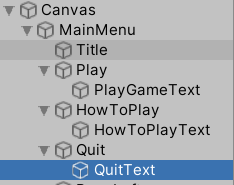
\includegraphics[width= 0.5\linewidth]{Images/MainMenuElements.PNG}
  \caption{Menu Elements.}
  \label{fig:MenuEle}
  \end{subfigure}%
  \begin{subfigure}{.5\textwidth}
\centering
  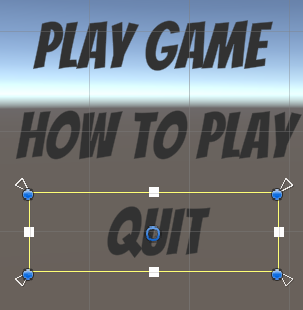
\includegraphics[width= 0.5\linewidth]{Images/TextBox.PNG}
  \caption{Quit Text Box in Yellow.}
  \label{fig:TextBox}
  \end{subfigure}%
\end{figure}
\newpage

\begin{figure}[h]
\centering
  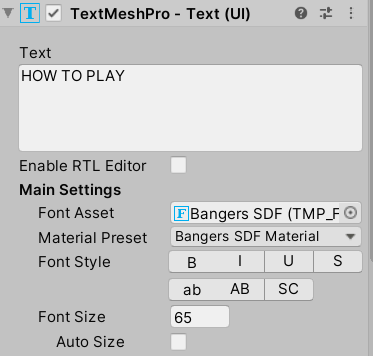
\includegraphics[width= 0.8\linewidth]{Images/TextEditor.PNG}
  \caption{Text Editor Example.}
  \label{fig:Text Editor}
\end{figure}

Each of the text boxes are children of a button function in which when pressed would lead to a new UI element. This is done by creating an on click function in the button field in the inspector, see figure \ref{fig:OnClick()}, where you would drag in the UI element you want and add a set active function to turn a UI element on or off by ticking a box. For example, if you click on the Play Game button, the Main Menu UI will be turned off and the Level Select UI will be turned on, allowing the player to see a new level select menu.
\begin{figure}[h]
\centering
  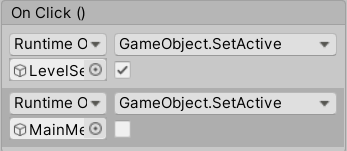
\includegraphics[width= 0.8\linewidth]{Images/OnClick.PNG}
  \caption{OnClick() function.}
  \label{fig:OnClick()}
\end{figure}
This is done for each different UI screen so that you can switch between them on the clicking the buttons so that there is no overlap of different UI's. For the Level Select UI however, in order for the buttons to be bring you to the different level scenes a script is needed in order to actually load the level scene you want to play. For this you would drag in the UI element that holds the script that is used to load the levels and set which method in the script you want to run that will load the desired scene. Below is a code snippet of the code required in order to load a level.
\begin{figure}[h]
\centering
  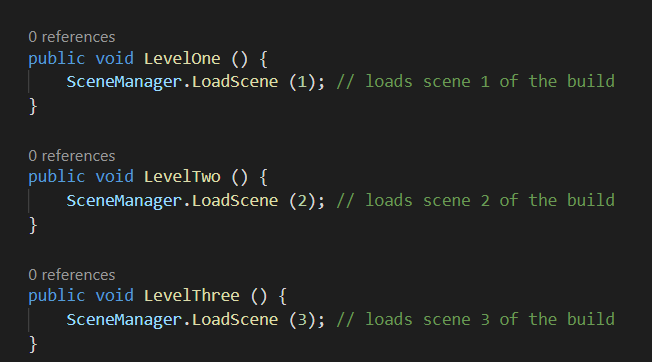
\includegraphics[width= 0.8\linewidth]{Images/LevelSelectCode.PNG}
  \caption{Code Snippet from MainMenu.}
  \label{fig:Level}
\end{figure}

\newpage
The same can be done for the the quit button on the main menu where the method for quitting the game is called which closes the application when being ran from the built version of the game. The code snippet below shows how this is done along with an extra line called Debug.log() which is used to test that the feature works when working from inside Unity through the console as when it is pressed while running the game in the game window, it wont actually exit the game as the application has not actually been made.

\begin{figure}[h]
\centering
\begin{subfigure}{.5\textwidth}
\centering
  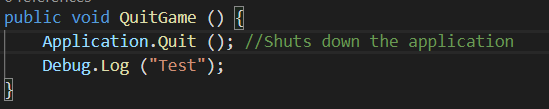
\includegraphics[width= 0.8\linewidth]{Images/Quit.PNG}
  \caption{Code Snippet for Quit();.}
  \label{fig:Quit}
  \end{subfigure}%
  \begin{subfigure}{.5\textwidth}
\centering
  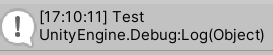
\includegraphics[width= 0.8\linewidth]{Images/QuitTest.PNG}
  \caption{Testing Quit in the console.}
  \label{fig:Debug}
  \end{subfigure}%
\end{figure}
\subsection{Final Menu View}
This subsection will be used to show how each menu UI turned out in the final build of the game.

\begin{figure}[h]
\centering
\begin{subfigure}{.5\textwidth}
\centering
  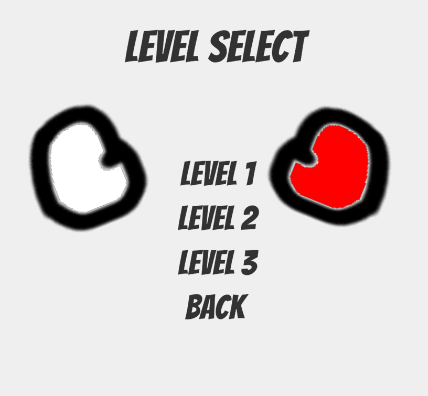
\includegraphics[width= 0.8\linewidth]{Images/LevelSelect.PNG}
  \caption{Level Select Menu.}
  \label{fig:LevelSelectMenu}
  \end{subfigure}%
  \begin{subfigure}{.5\textwidth}
\centering
  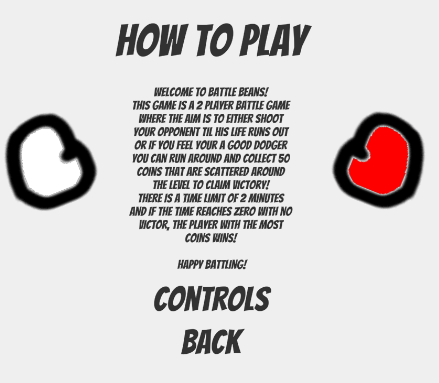
\includegraphics[width= 0.8\linewidth]{Images/How To Play.PNG}
  \caption{How To Play Menu.}
  \label{fig:HTP}
  \end{subfigure}%
  \newline
    \begin{subfigure}{.5\textwidth}
\centering
  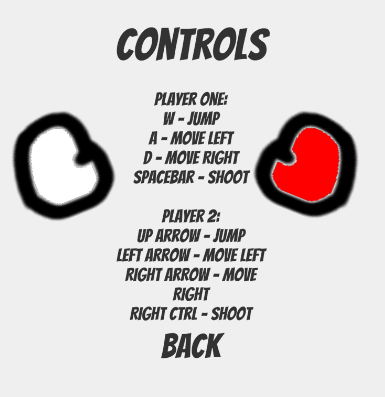
\includegraphics[width= 0.8\linewidth]{Images/Controls.PNG}
  \caption{Controls Menu.}
  \label{fig:Controls}
  \end{subfigure}%
\end{figure}
\newpage

\section{Level Design}
In this section I will go through the design of each of the three levels present in the final build of the game. I will be showing shots of the final build of the levels and how it was made as well as the sprites used to create the platforms, the items that can be picked up and how spawn points were made for coins and health.

\subsection{Sprites}
For the design of the levels, I put in simple sprites that I made using the image editor GIMP and how I added colliders and scripts to them so that they would provide functionality to the game. These will include how I made health items so that the players can regain their health, coin items so that a score could be gained from collecting them, the animations used and how I added colliders platforms and borders so that the players could not go through them.

\subsection{Environment Sprites}
As stated above, I used the image editing software GIMP, described in section 3.3.1, to create the sprites needed for the levels layouts. Once the images were created in GIMP, they were exported to PNG images for use in Unity. Once they were in Unity, a folder was created and named Sprites so that I could easily sort and find all the sprite images needed for development. To use the sprites, I simply clicked and dragged them into the scene view in Unity which would place them in the scene I was working on. Once they were added to the scene, I would add either a Box Collider 2D component or a Circle Collider which would put either an invisible box or circle around the sprite image so that the player character would not simply just slip through it and fall out of the level. The collider would then show a green outline to show the size of the collider added which could be edited by pressing the Edit Collider button in the inspector, see figure below, \ref{fig:Green} and \ref{fig:ColliderMenu}.
\begin{figure}[h]
\centering
  \begin{subfigure}{.5\textwidth}
\centering
  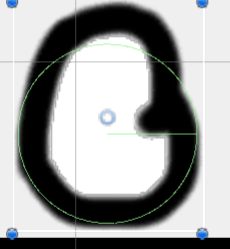
\includegraphics[width= 0.5\linewidth]{Images/ColliderOnObject.PNG}
  \caption{Example of green outline on Sprite.}
  \label{fig:Green}
  \end{subfigure}%
    \begin{subfigure}{.5\textwidth}
\centering
  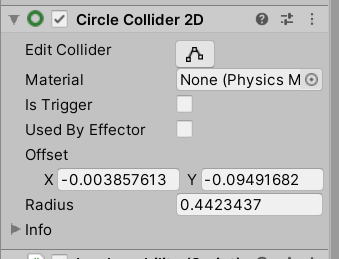
\includegraphics[width= 0.8\linewidth]{Images/ColliderInspector.PNG}
  \caption{Collider menu in Inspector.}
  \label{fig:ColliderMenu}
  \end{subfigure}%
\end{figure}
\newpage

For the levels platforms, as well as adding a box collider to them so that the player could stand on them without falling through, I added a feature that would allow the player to jump through the bottom of the platform allowing for easy access to collect the coins that would appear and allow the player to quickly escape the other player without getting trapped. I did this by adding a component called "Platform Effector 2D" which would allow you to create a surface arc of 180 degree and setting it to one way allowing the player to jump through the bottom but not slip through the top. Once this was added, a tick box would be selected in the box/circle collider to allow it to use the effector component which would enable it to work.

\begin{figure}[h]
\centering
  \begin{subfigure}{.5\textwidth}
\centering
  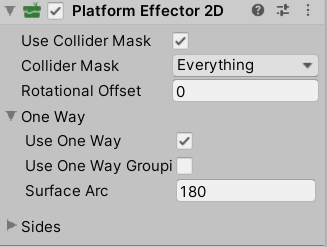
\includegraphics[width= 0.8\linewidth]{Images/PlatformEffector2D.PNG}
  \caption{Platform Effector.}
  \label{fig:PlatEffect}
  \end{subfigure}%
    \begin{subfigure}{.5\textwidth}
\centering
  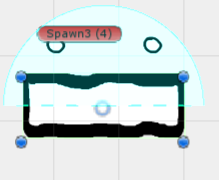
\includegraphics[width= 0.8\linewidth]{Images/PlatformWithEffector.PNG}
  \caption{Platform with effector on.}
  \label{fig:PlatEffOn}
  \end{subfigure}%
\end{figure}

\subsection{Using Scripts On Sprites}
For a couple of sprites, Scripts had to be added to provide functionality to them. These include the coins used to add up the players score, health items so that the player could regain lost health and a script to add functionality to the player sprite so that it could move, jump, shoot, take damage, etc. 

\subsection{Coins}

\begin{figure}[h]
\centering
  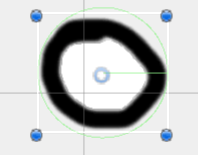
\includegraphics[width= 0.3\linewidth]{Images/Coin.PNG}
  \caption{Coin Sprite.}
  \label{fig:Coin}
\end{figure}

For the coins, I added a circle collider and set "Is Trigger" to be on as for the script I needed the collider to be a trigger so that when the players collider hit the coins collider it would register that the colliders had hit each other so that the method OnTriggerEnter2D in the Coin script could run, see Figure \ref{fig:CoinTrig}.

\begin{figure}[h]
\centering
  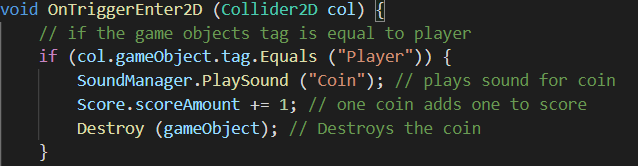
\includegraphics[width= 0.8\linewidth]{Images/CoinTrigger.PNG}
  \caption{Code Snippet from Coin.}
  \label{fig:CoinTrig}
\end{figure}

For this the coin would only react to a gameObject that contained the tag "Player", which is the tag given to the player gameObject. Once the coin recognized that it was the player that hit it, it would then add a value of 1 to the players score vale, more on this later, and then destroy itself so that it cant be continuously picked up with out actually disappearing, see figure \ref{fig:Health}.

\subsection{Health}
\begin{figure}[h]
\centering
  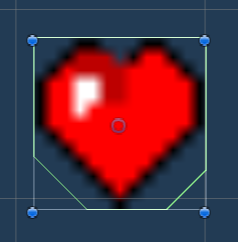
\includegraphics[width= 0.2\linewidth]{Images/Heart.PNG}
  \caption{Heart Sprite.}
  \label{fig:Heart}
\end{figure}
For the Heart and health, I added a Polygon Collider to it as this fits the sprite image itself, which is useful for sprites that are not circular or square, and also set this to have "Is Trigger" set to on similarly to the coin sprite. Like the coin sprite, the heart sprite also had a OnTriggerEnter2D method so that it could run when the the player game object with the tag "Player" collided with it.
\begin{figure}[h]
\centering
  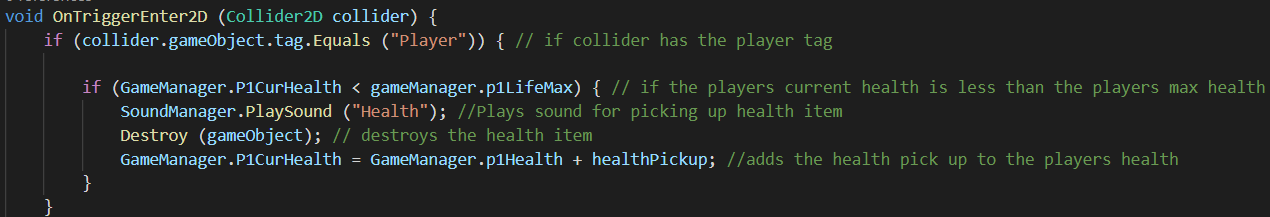
\includegraphics[width= 1\linewidth]{Images/HealthTrigger.PNG}
  \caption{Code snippet from HealthPickUp.}
  \label{fig:Health}
\end{figure}
\newline
Similarly to the coin script, when the player hit the heart sprite if the players health was lower than it's max health, it would add 1 health to the players current health but not if the player was already at max health. It would then destroy itself so that it couldn't be continuously picked up.


\subsection{Player}
\begin{figure}[h]
\centering
  
\includegraphics[width= 0.3\linewidth]{Images/Player.PNG}
  \caption{Player Sprite.}
  \label{fig:Player}
\end{figure}
For each player, a circle collider was added and a PlayerController script was attached to them to allow functionality to the player. Variables were made for moving left, moving right, jumping, shooting, movement speed and jump force. These variables could be set for each player by assigning them to buttons using the fields in the Inspector view, see figure \ref{fig:PlayerInspect}. Along with adding these variables, there was more added to let Unity know which prefab was being used to act as the projectile used as the bullet for shooting and a field to set what was considered the ground for the player.

\begin{figure}[h]
\centering
  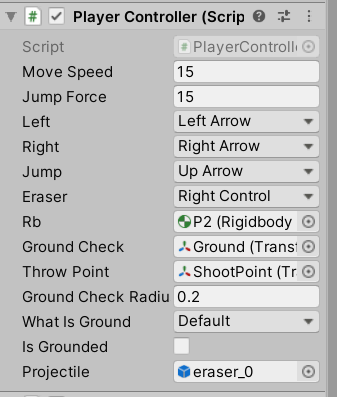
\includegraphics[width= 0.4\linewidth]{Images/PlayerControllerInspector.PNG}
  \caption{PlayerController Inspector view.}
  \label{fig:PlayerInspect}
  \end{figure}
\begin{figure}[h]
\centering
  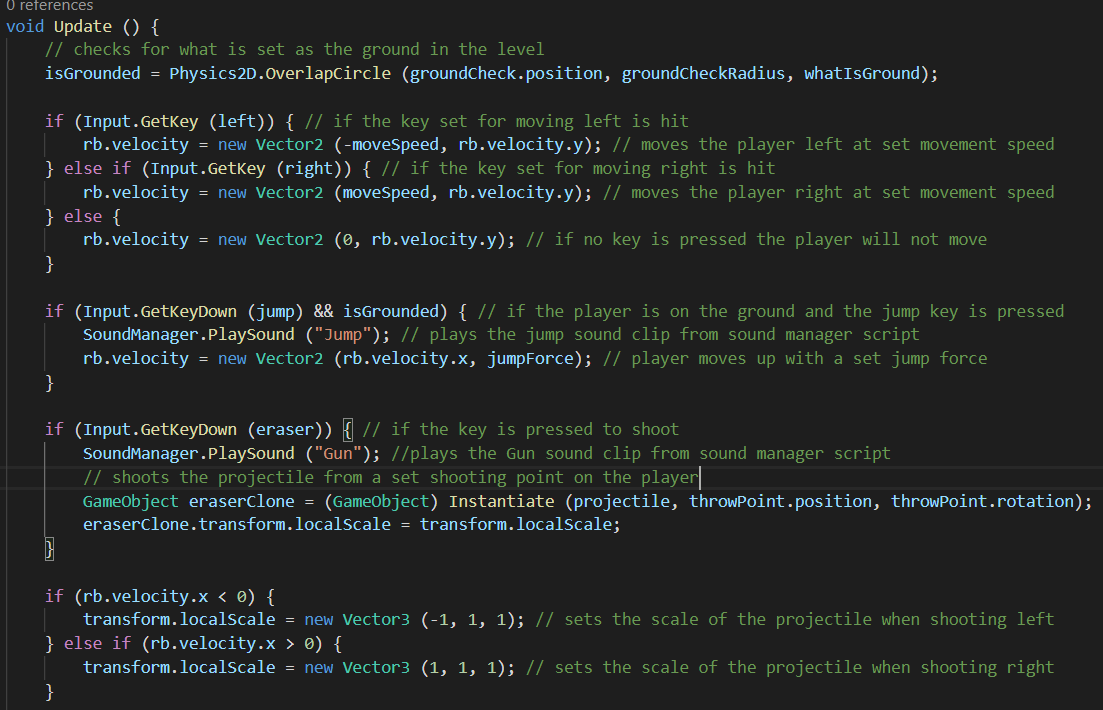
\includegraphics[width= 0.9\linewidth]{Images/PlayerController.PNG}
  \caption{Code Snippet From PlayerController.}
  \label{fig:PlayerControllerCode}
\end{figure}

Another script that was added to the player was the Invulnerability script which made it possible for the bullets to go straight through the player after being hit for 2 seconds. The reason this script was added was so that it gave the player a chance to get away from being attacked by the other player so that they wouldn't get spam shot meaning they would die very quickly. This was done by making the projectile layer ignore the player layer when the player was hit, making a transparent effect on the player for two seconds. It also meant that the player couldn't damage the other player while they were in the Invulnerable state as that would be unfair. See figure \ref{fig:Invulnerable}

\begin{figure}[h]
\centering
  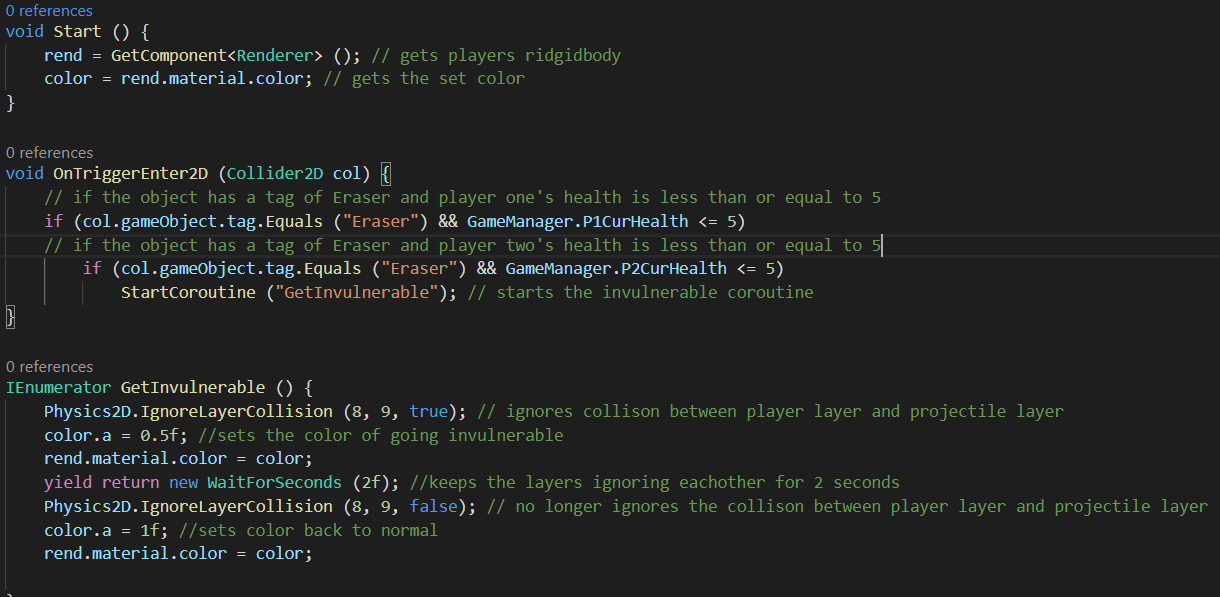
\includegraphics[width= 0.9\linewidth]{Images/Invulnerable.PNG}
  \caption{Code Snippet From Invulnerable.}
  \label{fig:Invulnerable}
\end{figure}
\newpage

\section{Game Manager}
The GameManager script was the biggest script involved in making the game as it contained ways for the players health to display as full and empty heart sprites to determine how much health a player had, how the player took damage, how to determine which winning screen it would show (Player one win screen or player two) and to be able to pause the game. This section will be used to describe how each of those mentioned above.

\subsection{Player Health System}
For the games health system, I decided to use a heart system similar to that in the Legend of Zelda games where a full heart represents 1 health and an empty heart represents health lost. To do this I set up two image arrays, one for a player one's hearts and one for player two's hearts. Then, using a for loop, I determined if the players health was less than the number of hearts. The number of hearts was set to be equal to the players health, so if one health was taken away it would mean that one full heart would be taken away and replace with an empty heart, see figure \ref{fig:Hearts}. I also set it so that the player can only have a number of 5 hearts in the inspector by setting max life to 5.
\begin{figure}[h]
\centering
  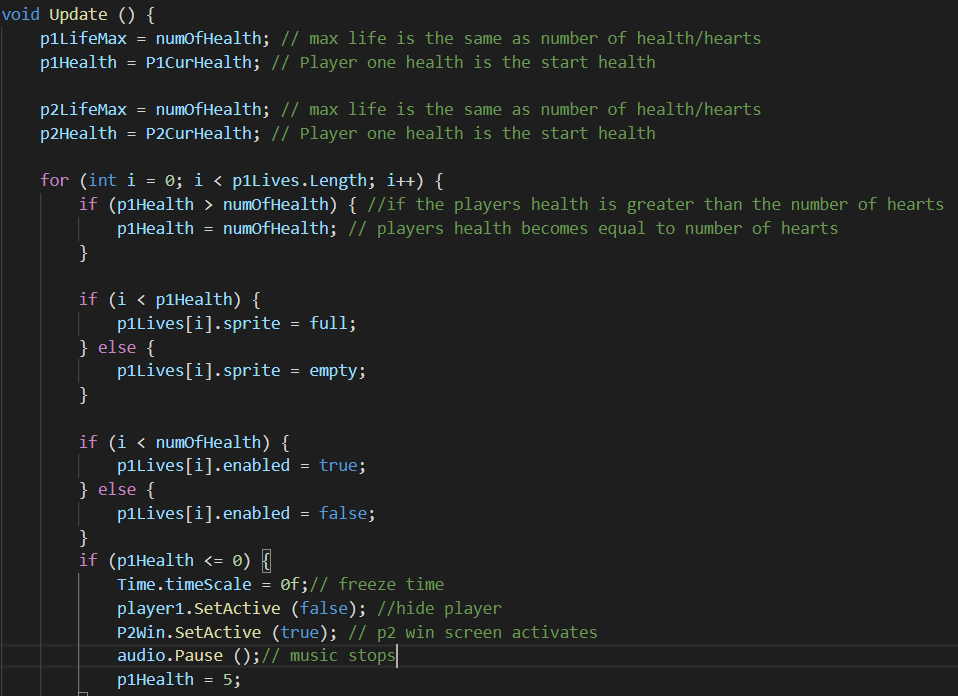
\includegraphics[width= 0.9\linewidth]{Images/HealthSystem.PNG}
  \caption{Code Snippet From GameManager.}
  \label{fig:GameManagerCode}
\end{figure}
\begin{figure}
\begin{subfigure}{.4\textwidth}
\centering
  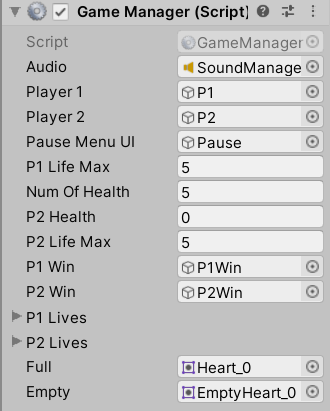
\includegraphics[width= 1\linewidth]{Images/GameManagerInspect.PNG}
  \caption{GameManager in the inspector.}
  \label{fig:GameManager}
  \end{subfigure}
  \begin{subfigure}{.5\textwidth}
\centering
  
\includegraphics[width= 1\linewidth]{Images/Hearts.PNG}
  \caption{Hearts Health system.}
  \label{fig:Hearts}
  \end{subfigure}
\end{figure}
\newpage

\subsection{UI Elements}
In this section I will be explaining how each of the player win screens, the pause screen, the draw screen, the score display and the timer display worked. Firstly for the the player wins screens, I added them very similarly to how I added all the elements to to the main menu UI in terms of adding text boxes to display "Player 1/2 Wins!!" and the buttons to go back to the main menu, seen in section 4.2. The main difference was that I had to add a snippet of code into the game manager to make the player win UI appear when a player brought the other players health down to zero. I also the same snippet of code to both the score scripts for when the players reached 50 points and for  the Countdown script so winner could be determined after the timer had reached 0. For when a players health reached zero, I made it so that when a players health would reach zero it would freeze the game using Time.timeScale function by setting it to 0. Then I would set the Player win UI element to active so that it would appear after either player one's or player two's health was equal to zero, as it is default set to be inactive. Below is a shot of the code snippet used to make this possible.

\begin{figure}[h]
\centering
  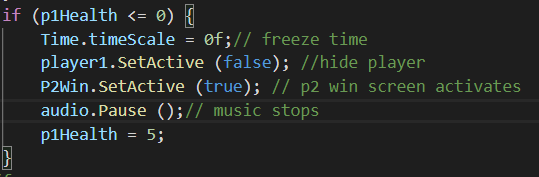
\includegraphics[width= 0.7\linewidth]{Images/P2Wins.PNG}
  \caption{Code Snippet For if player 2 wins.}
  \label{fig:P2Win}
\end{figure}

Similarly for both when a player reaches a score of 50 and determining a winner after the timer reaches 0, I wrote code for it to display the UI for each player winning as well as if the players had the same score after the timer finishes it would display a screen saying that the game had finished in a draw, with a button that on click would bring you back to the main menu. See below for code snippets of both Winning with score and getting the draw screen as well as determining a winner if the timer reaches 0.

\begin{figure}[h]
\begin{subfigure}{1\textwidth}
\centering
  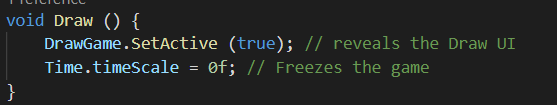
\includegraphics[width= 1\linewidth]{Images/Draw.PNG}
  \caption{Code Snippet for Draw.}
  \label{fig:Draw}
  \end{subfigure}
  \newline
  \begin{subfigure}{1\textwidth}
\centering
  \includegraphics[width= 1\linewidth]{Images/ScoreWinner.PNG}
  \caption{Code snippet for win at 50.}
  \label{fig:scorewin}
  \end{subfigure}
  \newline
    \begin{subfigure}{1\textwidth}
\centering
  \includegraphics[width = 1\linewidth]{Images/ScoreWinnersCountdown.PNG}
  \caption{Code snippet for a winner after timer hits 0}
  \label{fig:countdown}
  \end{subfigure}
\end{figure}

In order to bring up a pause screen, in the game manager I added a Boolean if the gameIsPaused is true or false and if it is true when to escape key is pressed it will display the pause menu. If the escape button is pressed again while in the pause menu, the Boolean will be returned to false and the pause menu will then become inactive, thus disappearing. Below is a snippet of code that enables the pause menu to appear along with how the pause menu looks.

\begin{figure}[h]
\begin{subfigure}{1\textwidth}
\centering
  \includegraphics[width= .4\linewidth]{Images/PauseMenu.PNG}
  \caption{Pause Menu UI.}
  \label{fig:PauseUI}
  \end{subfigure}
  \begin{subfigure}{1\textwidth}
\centering
  \includegraphics[width= 1\linewidth]{Images/PauseKey.PNG}
  \caption{Code snippet for Pause key.}
  \label{fig:escape}
  \end{subfigure}
  \newline
    \begin{subfigure}{1\textwidth}
\centering
  \includegraphics[width = 1\linewidth]{Images/Pause.PNG}
  \caption{Code snippet for pause methods}
  \label{fig:pause}
  \end{subfigure}
\end{figure}


For the timer, I added a text box to the middle top that displayed "0" and added a script to the canvas called Countdown. In this script I set variables for the Timer text, the current time and the start time. In the script I set the current time to be equal to the start time and in the Update() method i set the time to go down by one second every second until the timer had reached 0. once the timer had reached zero, I then set the current time to be zero so that it would stay at zero and then ran the winner method mentioned above for determining a winner based on score. Below is a snippet of code that shows how the timer works.
\begin{figure}[h]
\centering
  \includegraphics[width= 1\linewidth]{Images/Timer.PNG}
  \caption{Code Snippet For the timer.}
  \label{fig:Timer}
\end{figure}

\section{Spawning}
In this section I will briefly describe how I added spawnpoints for both the health items and the coins. To do this, I created two empty game objects called CoinSpawner and HealthSpawner and made children of both of these named spawn points. I then scattered the spawn points across each level and began writing a script for both the CoinSpawner and HealthSpawner. In these scripts I created arrays for both the spawnPoints and the items that will spawn at these points. Then I put an InvokeRepeating function in the start() method so that it would spawn the items at intervals of the given seconds, see figure \ref{fig:HealthSpawn} and \ref{fig:CoinSpawn}.A SpawnHealth/SpawnCoin method is then made to make the items spawn at the previously made spawn points at random. After the scripts where made, I dragged in the spawn points and the items into the correct fields displayed in the inspector, see figure \ref{fig:CoinSpawnInspect} and \ref{fig:HealthSpawnInspect}.

\begin{figure}[h]
\centering
  \includegraphics[width= .8\linewidth]{Images/SpawnPoints.PNG}
  \caption{Spawn Points on level in red.}
  \label{fig:SpawnPoints}
  \end{figure}

  \begin{figure}[h]
  \begin{subfigure}{1\textwidth}
\centering
  \includegraphics[width= 1\linewidth]{Images/HealthSpawn.PNG}
  \caption{Code snippet for HealthSpawn.}
  \label{fig:HealthSpawn}
  \end{subfigure}
  \begin{subfigure}{1\textwidth}
\centering
  \includegraphics[width = 1\linewidth]{Images/CoinSpawn.PNG}
  \caption{Code snippet for CoinSpawn}
  \label{fig:CoinSpawn}
  \end{subfigure}
  \begin{subfigure}{.5\textwidth}
\centering
  \includegraphics[width = 1\linewidth]{Images/CoinSpawnInspector.PNG}
  \caption{Coin spawn in the inspector}
  \label{fig:CoinSpawnInspect}
  \end{subfigure}
  \begin{subfigure}{.5\textwidth}
\centering
  \includegraphics[width = 1\linewidth]{Images/HealthSpawnInspector.PNG}
  \caption{Health spawn in the inspector}
  \label{fig:HealthSpawnInspect}
    \end{subfigure}
  \end{figure}
  
  



\chapter{System Evaluation}
After completing the development of my game, I had to look at evaluating its overall performance. The aim was to evaluate the game in the following areas:
\begin{itemize}
\item Robustness
\item Testing
\item Limitations
\item Results vs Objectives
\end{itemize}

\section{Robustness}
To measure the robustness of the game, I had decided to focus on this part of evaluation during the design and development of the project. I looked at the usability of the game itself in terms of the players control like jumping, moving and shooting, the UI elements appearing and disappearing when they should and in addition I gave friends a final build version of the game to test out.

\section{Testing}
Through using testing methods of white box testing and black box testing, I found that the project had reached a level design and functioning I had hoped for in the beginning when I set out to make this game. For white box testing, I tested the game myself in order to make sure everything was working the way that it was supposed to and that there were no major errors coming up on the console when running the game. For black box testing, I gave several different versions of builds to my friends to see if there where any bugs or problems playing the games. This allowed me to find any problems within the game that I may not have ran into when I was play testing the game myself.

\section{Limitations}
After the final build, which I sent to my friends to test out, it was discovered that there was an issue where if a player won the game by bringing the other players health down to zero and then went back to the main menu and started another game, the bullets would just go straight through the player and not damage them. After several hours of trying to fix the problem, I found no success. I came to the conclusion that it was not working because when the players health reached zero, it would stay at zero even though the hearts would show that the player had full health.

\section{Results V Objectives}
In the beginning, I had set out a number of objectives. In this section I will expand on these objectives. The project was made with the following objectives in mind:

\bigskip

\textbf {Make a Simple, yet fun to play game:} I feel that I did produce a fun simple game to play. After receiving feedback from the people I got to test the game they felt that it was a nice fun easy game to play around with. Using Unity made everything relatively easy as most things I had struggled with had tutorials on the unity website to help me along the way and it allowed me to provide a fun game.
\newline

\textbf {Dive into deeper learning into using game engines:} For the research part of the project I learned a lot about each different game engine and found that they are all great in their own way and I also now know which game engines to use in the future whether I will make a 2d game or a 3d game and which engine would produce the best results for my tastes.
\newline

\textbf {Complete the project using an efficient and effective approach:} As I had never done a project at this scale, I wanted to make sure I had all my ideas for the game finalized before I began working on the project. With being able to meet with my supervisor on a weekly basis or being able to contact him through email if for whatever reason I could not make the meeting was great in order to get feedback on my idea's and progress in the project.
\newline

\section{Overall Evaluation}
Overall, the game works as mostly intended and functions as a small fun game to play with a friend and it met my requirements that I set out in section 1.1 project objectives. Based on the tests I carried out by giving different build versions to friends, I was able to find bugs that I had not seen and fix them throughout development. Although I could have added improvements to the game like more levels or more characters, I was overall happy with the progress that I had made by the end. 


\chapter{Conclusion}
\section{Overview}
This report discussed the development of a small 2 player battle style game using the Unity game engine, whilst adopting an agile development methodology approach. From the beginning my main aim was to make a small battle game that would be fun and easy to play, but to also expand my knowledge when it came to games development. I wanted to be able to expand on the knowledge I had gained in making games throughout the 4 years of the software development course. In summary, the main objectives for this project was outlined as:
\newline
\begin{itemize}
\item Introduce the concept of the project
\item Provide an understanding of Game engines
\item Describe the development of the applied project
\item Make a simple, yet fun to play game
\item Dive into deeper learning into using game engines
\item Complete the project using an efficient and effective approach
\end{itemize}

From the evidence found that was discussed in chapter 6 System evaluation demonstrates that the original objects set out at the beginning have been achieved. I feel I provided a sufficient clear insight into games development to the reader.
The game allows for two players to play at the same time with both having their own separate inputs for moving, jumping and shooting. It also allows a winner to be determined through either reducing one players health to zero, reaching a score of 50 from collecting coins or having a higher score than the opponent when the timer reaches zero. Although this type of game doesn't seem new or inventive, I still believe it is a fun game to play much like other battle style games that are out there in the vast industry of video games.
\newline
In terms of requirements stated in section 1.4 Requirements, the end product complies with all the initial requirements specified. The game hits all the check boxes I feel it needed for it to be a fun short 2D 2 player game, allowing a small rest from reality and generally just to have fun.

\section{Learning Outcomes}
Throughout the scope of the project from start to finish, I have gained a substantial amount of new knowledge in the field of games development. From initial research and design to learning all the capabilities that Unity had to offer as well as some other game engines like Unreal Engine 4. The skills obtained and experiences earned will hopefully help me in the future if I can get into the career of video games development. My research gave me the ability to explore the present state of the process to make a video game. I have now seen first hand the importance of evaluating the work and research required to complete a project of this scale.
\newline
The skills learned have been priceless throughout the completion of the project. Even from researching how to do certain things on unity led me to see that there are so many ways to do one thing differently as all the developers out there have shown there own way of doing things and even I ended up doing certain things with my own kind of simpler twist on them. This module has also thought me how important meetings are in order to ensure that the deadlines can be met in time.

\section{Final Thoughts}
As the end of my 4 years in the Software Development course of GMIT is edging closer, I can happily hand up this project with a smile on my face and a sense of satisfaction in completing my goals. Even though I am no artist, I am happy with the way the game turned out after drawing my own art in a sketch art style as its not supposed to look good. The project was challenging from start to finish but reaching the end goal was such a rewarding experience and definitely a good way to get a feel of how the games industry works.

\section{A Word From The Developer}
 \textit{"I began studying programming 6 years ago in GTI for a games development course and i remember just getting a game to work without actually writing a line of code and thinking it was amazing. Fast forward to now where I was able to get a full game with code working all on my own, its still hard to believe. There has been a lot of struggles and late nights leading up to now but now that I'm nearing the end of the road I can safely say I have no regrets. This project could not have been done without the never ending help from my supervisors Dr. John Healy and Kevin O'Brien, they have my thanks. To whoever ends up playing this game, i hope it gives you even a little bit of fun, as the aim of this game from the start was to give the player just a bit of fun!"}
\chapter{Appendices}

\textbf {GitHub:} \newline \bigskip
\href{https://github.com/Doylers123/Y4FYP}{https://github.com/Doylers123/Y4FYP}

\textbf {GitHub Main Project:} \newline \bigskip
\href{https://github.com/Doylers123/Y4FYP/tree/master/New\%20Unity\%20Project}{https://github.com/Doylers123/Y4FYP/tree/master/New\%20Unity\%20Project}

\textbf {Video Presentation:} \newline \bigskip
\href{https://www.youtube.com/watch?v=4Sa85aqMVlk}{https://www.youtube.com/watch?v=4Sa85aqMVlk}

%----------------------------------------------------------------------------------------
\bibliographystyle{unsrt}
\bibliography{references.bib}

\end{document}